Les techniques d'approximation d'EDPs d'évolution comportent souvent une étape nécessitant la résolution d'une équation différentielle ordinaire
\footnote{On utilisera aussi le terme \textit{système dynamique}, même si en toute rigueur ce concept est un peu plus large.} (EDO),
c'est à dire une équation différentielle ne faisant intervenir qu'une seule variable différenciée, généralement le temps. Cette section rappelle 
quelques notions d'analyse et de simulation des EDOs du premier ordre.\par

\begin{definition}[Équation différentielle ordinaire]
    Une équation différentielle ordinaire (du premier ordre) est une équation de la forme :
    \begin{align}\label{def:def_ODE}
        u' &= A(u,t)\quad u : t \in \mathbb{R}^+ \mapsto u(t) \in \mathbb{R}^d\\\notag
        u(0)&=u_0 \in \mathbb{R}^d.
    \end{align}
\end{definition}
%%%%%%%%%%%%%%%%%%%%%%%%%%%%%%%%%%%%%%%%%%%%%%%%%%%%%%%%%%%%%%%%%%%%%%%%    SCHEMA EXPLICITES ET IMPLICITES
\subsection{Schémas explicites et implcites.}
L'approximation des EDO se fait grâce à des schémas numériques, c'est à dire une suite d'élément $(u^n)$ de $\mathbb{R}^d$.
Donnés une EDO et un pas de discrétisation temporel $\Delta t$, $u^n \mathbb{R}^d$ est approxime la solution de l'EDO au temps $t^n = n \Delta t$.
C'est à dire que la suite $(u^n)_{n\in \mathbb{N}} \in (\mathbb R^d)^\mathbb{N}$ définie par un schéma numérique cherche à avoir à avoir $u^n \approx u(t=n\Delta t)$.
Deux catégories de schémas numériques existent: les schémas explicites et les schémas implicites
% Seuls les schémas à un pas sont ici présentés et non pas les schémas multi-pas. Ce choix est fait en raison de la barrière de Dahlquist
% \footnote{\url{https://fr.wikipedia.org/wiki/Methode_lineaire_a_pas_multiples\#Premiere_et_deuxieme_limites_de_Dahlquist}}.


\begin{definition}[Schéma explicite]
    Un schéma numérique est dit explicite si le pas de temps $n+1$ est obtenu seulement grâce au pas de temps $n$, usuellement formulé sous la forme:
    \begin{align}
        u^{n+1} = u^n + f(u^n ,\Delta t ).
    \end{align}
\end{definition}

\begin{definition}[Schéma implicite]
    Un schéma numérique est dit implicite si le pas de temps $n+1$ est obtenu au moins en partie grâce au pas de temps $n+1$, souvent écrit comme:
    \begin{align}
        u^{n+1} = u^n + f(u^{n+1} ,\Delta t ).
    \end{align}
    Ainsi, une itération d'un schéma implicite nécessite l'inversion d'un système linéaire ou non linéaire. 
\end{definition}
De fait une itération implicite est souvent plus coûteuse qu'une itération d'un schéma explicite
\footnote{En particulier si la dimension de la solution $d$ est grande.}. 
Cependant pour des raisons de stabilités (voir \ref{par:stabilite_edo}) les méthodes explicites peuvent nécessiter des pas de temps bien plus fin, et donc bien plus d'itérations.
Le choix entre méthode explicite et implicite dépend de bien des facteurs (du problème, du niveau de précision voulu, de la difficulté d'implémentation etc...)
c'est un enjeu central de la simulation numérique.
%%%%%%%%%%%%%%%%%%%%%%%%%%%%%%%%%%%%%%%%%%%%%%%%%%%%%%%%%%%%%%%%%%%%%%%%
\subsection{Ordre d'un schéma}
La notion d'ordre de convergence permet de lier l'erreur d'une solution numérique au pas de temps utilisé, en clair cela quantifie l'efficacité d'un schéma numérique.
\begin{definition}[Erreur locale d'un schéma]
    L'erreur locale d'un schéma numérique de résolution d'une EDO est l'erreur que commet le schéma sur un pas de temps.
    Autrement dit si l'on note $u$ la solution de l'EDO à partir d'un état initial $u_0 = u(t=0)$ et $u_1$ l'approximation numérique proposée par la schéma 
    pour un pas de temps $\Delta t$ à partir de l'était $u_0$, l'erreur locale est: 
    \begin{align}
        e(\Delta t) = \Vert u(\Delta t) - u_1 \Vert.
    \end{align}
\end{definition}

\begin{definition}[Erreur globale d'un schméa]
    L'erreur globale d'un schéma est l'erreur que commet le schéma sur plusieurs pas de temps. 
    Si l'on note $u^n$ la solution numérique au temps $t^n = n \Delta t$, alors l'erreur globale du schéma jusqu'au temps final $T = N \Delta t$ peut être définie comme:
    \begin{align}
        E(\Delta t) = \sum_{n=0}^N \Vert u^n - u(n^t) \Vert 
    \end{align}
    ou plus simplement encore:
    \begin{align}
        E(\Delta t)=\Vert u^n - u(T) \Vert.
    \end{align}
\end{definition}

\begin{definition}[Ordre de convergence]
    Un schéma numérique de résolution d'une EDO est dit d'ordre $p$ si de manière équivalente:
    \begin{itemize}
        \item[$\diamond$] L'erreur locale vérifie : $e(\Delta t) = O(\Delta t^{p+1})$
        \item[$\diamond$] L'erreur globale vérifie : $E(\Delta t) = O(\Delta t^{p})$
    \end{itemize}
\end{definition}

%%%%%%%%%%%%%%%%%%%%%%%%%%%%%%%%%%%%%%%%%%%%%%%%%%%%%%%%%%%%%%%%%%%%%%%%
\subsection{Stabilité des schémas numériques}\label{par:stabilite_edo}
Un schéma numérique d'ordre $p$ converge vers la solution exacte de l'EDO avec une erreur qui décroît asymptotiquement en $\Delta t^p$ lorsque le pas de temps diminue.
Cependant, cette convergence n'est garantie que si le schéma reste stable.
L'instabilité d'un schéma désigne la divergence de la solution numérique : au-delà d'un pas de temps critique $\Delta t_0$, la norme de la solution discrète $\|u^n\|$ tend vers l'infini\footnote{Phénomène communément appelé "explosion" de la solution numérique.}.
Cette instabilité peut s'interpréter de deux manières complémentaires : d'un point de vue mathématique, le schéma se comporte comme une suite géométrique de raison $|r| > 1$ ; 
d'un point de vue physique, le schéma introduit artificiellement de l'énergie dans le système à chaque itération.
La contrainte de stabilité impose donc la contrainte $\Delta t < \Delta t_0$. 
Lorsque ce seuil $\Delta t_0$ est très restrictif, c'est à dire très faible, la résolution de l'EDO nécessite un nombre d'itérations $T_{\text{final}}/\Delta t$ important,
ce qui augmente considérablement le coût calculatoire. 
Les schémas explicites sont généralement plus prompts aux instabilités que les méthodes implicites.
\begin{figure}[htbp]
    \centering
    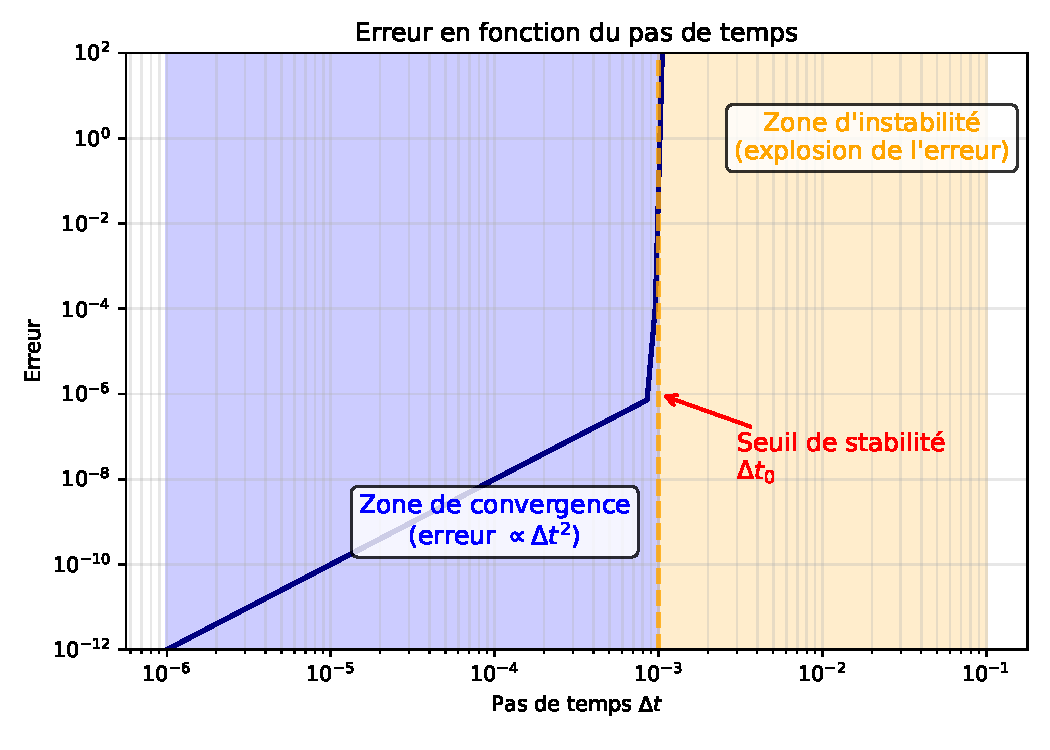
\includegraphics[width=0.8\textwidth]{media/3_/2_/exemple_satabilite.pdf}
    \caption{Illustration du comportement attendu de l'erreur d'un schéma d'ordre deux dont le seuil d'instabilité serait $\Delta t > 10^{-1}$.}
    \label{fig:stabilite_schema}
\end{figure}
\begin{definition}[Stabilité d'un schéma numérique]
    Un schéma numérique $\bigl( u^n \bigr)_{n \in \mathbb{N}} \in\bigl(\mathbb{R}^d \bigr)^{\mathbb{N}}$ est stable si et seulement si :
    \begin{align}
        \Vert u^{n+1} \Vert \leq \Vert u^n \Vert.
    \end{align}
    Cette condition est souvent vérifiée à la condition que le pas de discrétisation $\Delta t$ n'excède pas un seuil de stabilité $\Delta_0$ fonction de l'ODE et le schéma d'intégration.
\end{definition}
La stabilité d'une méthode d'intégration d'EDO dépend entre autres de l'opérateur intervenant dans l'équation (le $A$ dans l'équation \ref{def:def_ODE}).
Un opérateur tendant à poser des problèmes de stabilité est dit raide.
\begin{definition}[Problème raide]
    Un système dynamique, est dit raide si les méthodes explicites ne sont pas adaptées à sa résolution.
    En termes plus mathématiques le système:
    \begin{align}
    \frac{\text d u}{\text{d}t} = A(u,t), \quad u(t) \in \mathbb{R}^d, \forall t\geq 0.
    \end{align}
    est dit raide si la jacobienne de $A$, $J_A$ possède des valeurs propres négatives de grande amplitudes devant les autres valeurs propres.
    Si tel est le cas, plusieurs relaxations sont mises en jeu mais chacune avec des temps caractéristiques d'ordres de grandeur différents.
    Pour les méthodes explicites, si le pas de temps n'est pas assez petit, la relaxation rapide est mal résolue et
    impose un gradient fort trop longtemps (le gradient devrait s'atténuer, mais à une échelle trop rapide pour être captée pour le pas de temps du schéma) ce qui 
    déstabilise la méthode.
\end{definition}
En simplifiant, si un opérateur est raide, il impose une condition de stabilité très restrictive aux méthodes explicites et 
force à choisir des méthodes implicites\footnote{La réalité est plus nuancée, nous le verrons.}.
\begin{exemple}[Équation de Dahlquist]
    Pour saisir de manière plus intuitive le concept de raideur, prenons le cas de l'équation de Dahlquist
    \footnote{C'est le cas le plus simple d'une valeur propre négative}:
    \begin{align}
        \frac{\text d u }{\text d t} &= - \lambda u,\quad \lambda > 0\\\notag
        u(t=0)&=u_0
    \end{align}
    La solution analytique est : $u(t) = u_0 e^{-\lambda t}$. Ainsi passé quelque $ 1/\lambda$ la dynamique du système est au point mort. 
    En pratique la dynamique digne d'intérêt du système se concentre donc entre $t=0$ et $t=\frac{10}{\lambda}$. 
    Au delà, $u(t>\frac{10}{\lambda}) = o(u_0)$, la dynamique est terminée.
    Ainsi, si l'on souhaite simuler le comportement d'un tel système, il faut choisir des pas de temps petits devant $\vert \lambda \vert^{-1}$.
    Lorsque $\lambda$ est de grande amplitude cela devient très contraignant... Si l'on souhaite utiliser des méthodes explicites, c'est encore pire car la raideur du système 
    n'est plus une simple contrainte de précision mais de stabilité. En effet si l'on cherche à approximer le système par un schéma d'Euler explicite, alors : 
    $U^{n+1} = U^n (1 - \lambda \Delta t)$ alors la contrainte de stabilité est $\Delta t \, \lambda < 1/2$ ce qui est contraignant si $\lambda$ est grand. 
    Si $\lambda = 10^5$ alors il faut avoir $\Delta t \approx 10^{-5}$ donc pour simuler le système entre $t=0$ et $t=1$ il faut cent mille points !
    A l'inverse si l'on choisit un schéma d'Euler implicite: $u^{n+1} = u^n - \lambda \Delta t u^{n+1}$, alors la condition de stabilité devient : 
    $\Vert(1+\lambda \Delta t)^{-1}\Vert \leq 1$ ce qui est toujours vrai, quelque soit $- \lambda \in \mathbb{R}^-$, la raideur du système n'est pas un problème pour la méthode implicite.
    On comprend mieux la définition précédente \textit{Un système dynamique, est dit raide si les méthodes explicites ne sont pas adaptées à sa résolution.}
\end{exemple}
Il existe différents types de stabilité comme la A-stabilité (méthode stable indépendamment de la raideur du problème), la L-stabilité (schéma amortissant les hautes fréquences),
par souci de concision cette partie s'achève ici mais ces notions sont développées par exemple dans \cite{HairerAndWanner1}.